% On the other hand, assuming purely rigid motions is a strong restriction that is barely fulfilled in organic shapes. When a person moves, there are parts of their body moving rigidly (e.g. upper and lower arms or legs) and others which are transitions between the rigid ones (e.g. the neck). Be- sides, rigid motions within a fine-grained articulated struc- ture may not be observable with the limited resolution of a camera. For these reasons, a sharp segmentation will never be able to estimate the motion of life beings or some other inanimate objects with exactitude.

%TODO: think about where to explain the difference between rigid-and deformable motion.



\chapter{Introduction}
\section{Motivation}
In nature one important aspect that determines the odds of survival and thus the individual success to reproduce is the ability to sense the surrounding environment. In particular, the perceptional system of any advanced species is directed by visual cues amongst others. Alongside with sensing color, depths and brightness, the perception of motion is a fundamental visual cue. Particularly, motion is of great importance for interpreting visual information such as object groupings and their structure, estimating speed and performing self-localization, as shown in Figure $\ref{fig:motivating_example}$.
\begin{figure}[H]
\begin{center}
\subfigure[Sensing Depths and Localization]{
   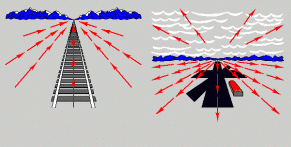
\includegraphics[width=0.31\linewidth] {introduction/motivation/perception/orientation}
   \label{fig:motivating_example_a}
}
\subfigure[Sensing Speed]{
   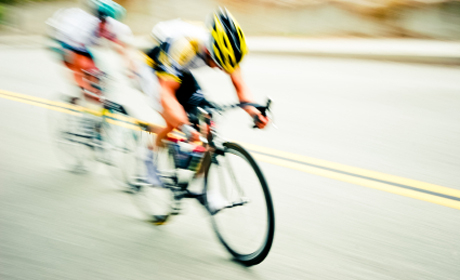
\includegraphics[width=0.31\linewidth] {introduction/motivation/perception/speed}
   \label{fig:motivating_example_b}
}
\subfigure[Temporal Grouping]{
   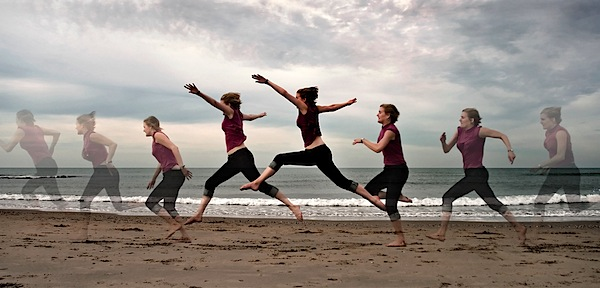
\includegraphics[width=0.31\linewidth] {introduction/motivation/perception/content}
   \label{fig:motivating_example_c}
}
\subfigure[Grouping Moving Objects]{
   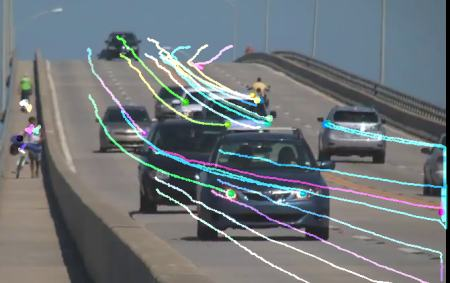
\includegraphics[width=0.31\linewidth] {introduction/motivation/perception/motion_tracking}
   \label{fig:motivating_example_d}
}
\end{center}
\caption[Motivating Example]{Motivating Examples$\footnotemark$: Visual cues allow us to group objects, estimate speed and depths and perform self-localization}
\label{fig:motivating_example}
\end{figure}
\footnotetext{Source Figure \ref{fig:motivating_example_a}: \url{http://opticflow.bu.edu/} \\
 source Figure \ref{fig:motivating_example_b}: \url{http://practicalphysics.org/forces-and-motion.html} \\
 source Figure \ref{fig:motivating_example_c}: \url{http://digital-photography-school.com/a-beginners-to-capturing-motion-in-your-photography/} \\
 source Figure \ref{fig:motivating_example_d}: \url{http://docs.opencv.org/trunk/d7/d8b/tutorial_py_lucas_kanade.html}}
Despite its apparent simplicity, motion is a very general and powerful cue to detect moving objects or even to partition them into their logical parts. This kind of object separation is also known as \textit{motion segmentation}. Generally, moving objects can be identified independently of their shape, type or looks. For instance it does not matter whether or not an object represents an animal or a car, both can be segmented by their motion. \\ \\
As natural such tasks might be performed by our brains the harder they become to realize in a technical point of view. Especially the task of an accurate detection and extraction of the moving objects in a video, captured by a moving camera, is nowadays still a very challenging problem. \\ \\
However, a lot of scientific effort has been put into solving this problem statement and many sophisticated approaches have been established. In particular, the most promising motion segmentations were produced by methods relying on optical flow fields. An example is given in Figure $\ref{fig:motion_segmentation_motivation_eg}$.
\begin{figure}[H]
\begin{center}
\subfigure[Optical Flow Field]{
   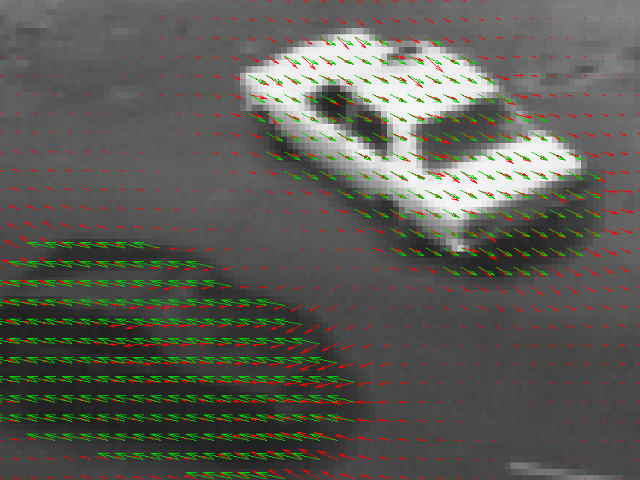
\includegraphics[width=0.47\linewidth] {introduction/motivation/motion_segmentation/optical_flow_visualization}
   \label{fig:motion_segmentation_motivation_eg_a}
}
\subfigure[Motion Segmentation]{
   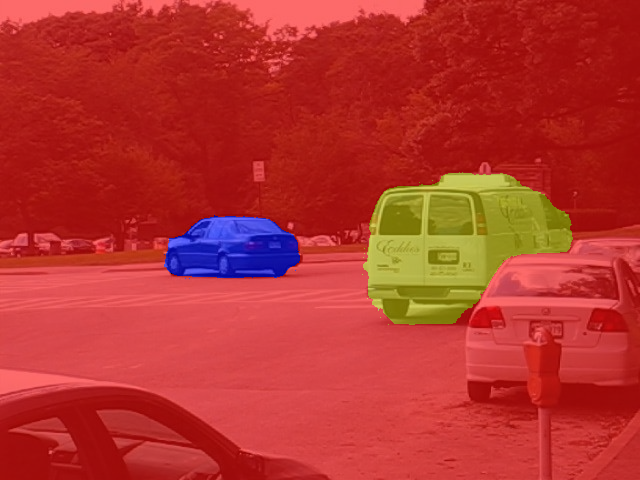
\includegraphics[width=0.47\linewidth] {introduction/motivation/motion_segmentation/dense_motion_segmentation}
   \label{fig:motion_segmentation_motivation_eg_b}
}
\end{center}
\caption[Motion Segmentation Motivation Example]{An example$\footnotemark$ of an optical flow field and a motion segmentation. }
\label{fig:motion_segmentation_motivation_eg}
\end{figure}
\footnotetext{Source Figure \ref{fig:motion_segmentation_motivation_eg_a}: \url{http://cbia.fi.muni.cz/projects/optical-flow-for-live-cell-imaging_3.html} \\
 and source Figure \ref{fig:motion_segmentation_motivation_eg_b}: \url{http://lmb.informatik.uni-freiburg.de/research/segmentation/}}
The field of motion segmentation aims at decomposing a video into moving objects and background and is the first fundamental step in many computer vision algorithms. It has many applications in the fields of robotics, metrology, video surveillance and traffic monitoring. \\ \\
The idea of using optical flow fields as an estimate of the motion goes back to the pioneering work of B. Horn and B. Schunck $\cite{Hs81}$. In this thesis we will build upon the body of work $\cite{Bro11a}$, $\cite{OB14b}$ and $\cite{KB15b}$ from T.Brox, who promotes an approach based on clustering trajectories extracted via optical flow. \\ \\
In combination with color, depth is another powerful visual clue that can be used to generate motion segmentations. A common technique is to segment objects according to their depth layer as described in $\cite{Dahan2012}$. However, most such techniques assume the presence of depth measurements. \\ \\
 Until recently, measuring depths in videos was rather unpractical since it required dedicated and expensive capturing devices and additional post-processing. However, with the advent of Microsoft's Kinect and other low price devices, RGB-D$\footnote{The term \textit{RGB-D} refers to color images with associated depth field measurements.}$ videos have become readily available. \\ \\
While combining RGB-D data with optical flow estimation has gained a lot of attention recently $\cite{Bro14}$, $\cite{PawanKumar2008}$ standard motion segmentation approaches have not yet been extended to benefit optimally from additional depth information. Therefore this thesis investigates this particular problem in detail and provides a solution for segmenting moving objects using optical flow fields on RGB-D videos.

% TODO: fix me: The purpose of this thesis is to describe and evaluate a robust motion segmentation method that incorporates depth information available in RGB-D video sequences as well as other visual cues.
\section{Goals}
The purpose of this thesis is to describe and evaluate a robust motion segmentation method and to incorporate depth information available in RGB-D video sequences as well as other visual cues. Due to its relative simplicity and extendibility we focus on motion segmentation with a traditional trajectory clustering approach using trajectories established via optical flow. In our formulation we assume a piecewise rigid motion$\footnote{A rigid motion can be represented by a transformation consisting of rotations and translations.}$ model and do not constrain the camera movement. \\ \\
The actual problem we want to address is shown in Figure $\ref{fig:problem_statement}$. For a given RGB-D video sequence and the camera calibration data, we want to detect and extract the individual moving objects. We therefore develop a pipeline that is capable of generating such motion segmentations by using optical flow fields. \\ \\
\begin{figure}[H]
\begin{center}
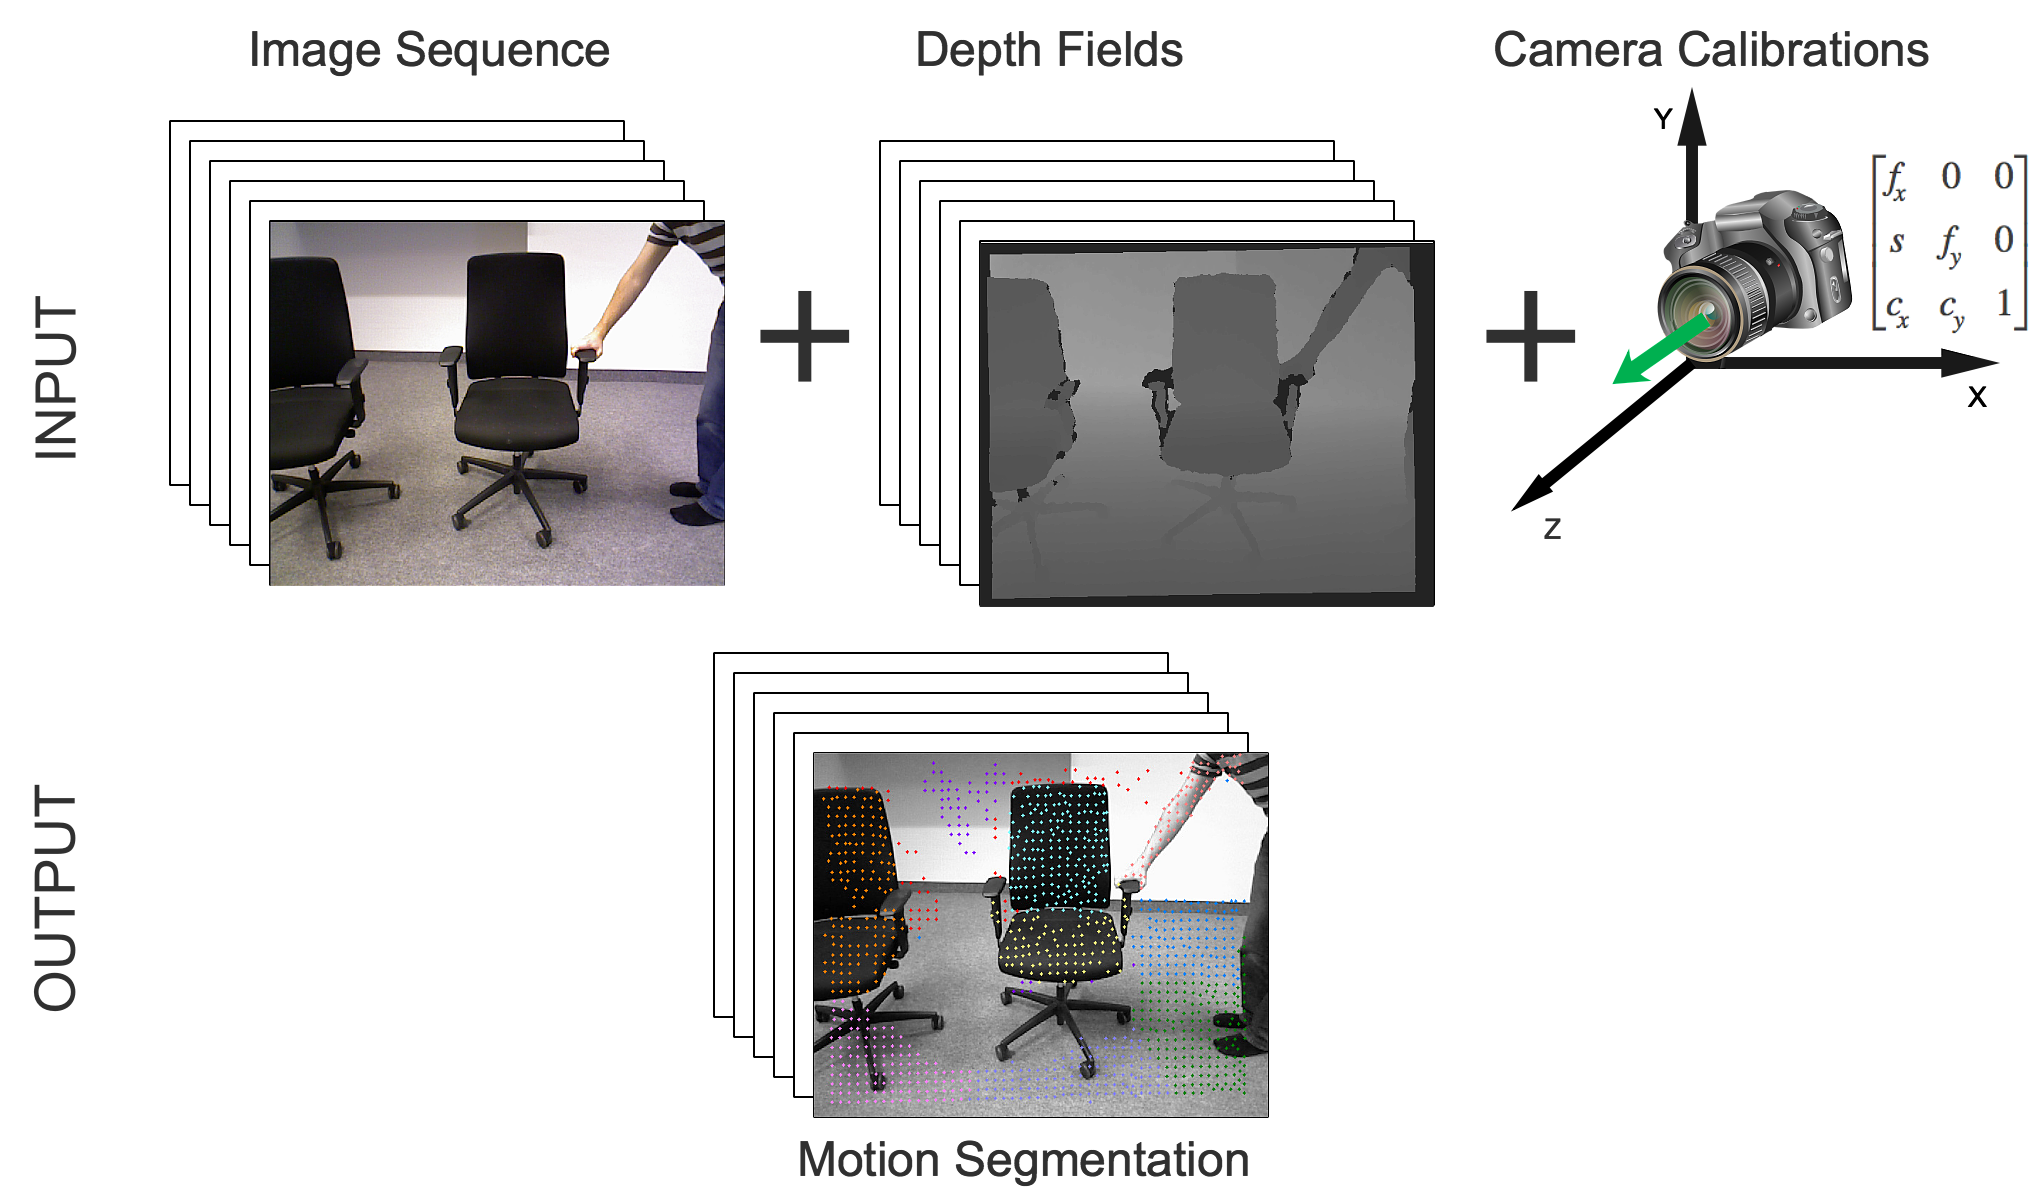
\includegraphics[width=1.05\linewidth] {introduction/problem_statement_ref}
\end{center}
\caption[Problem Statement]{ Graphical representation of the problem statement we want to solve in this thesis. Given a video sequence, its corresponding depth fields and the used camera calibrations, we want to extract the frames locations that mask the moving objects via segmentation.}
\label{fig:problem_statement}
\end{figure}
Moreover, we want to examine the influence of the utilized pipeline components. Hence, we integrate various segmentation- and flow-techniques into our implementation. We then quantitatively evaluate segmentations generated by all possible pipeline combinations. \\ \\
In summary, we want to achieve the following three goals:
\begin{itemize}
  \item Implement a pipeline that can segment moving objects by clustering trajectories established via optical flow and depth cues.
  \item Examine the influence of the used flow fields, the method of trajectory analysis and segmentation and how they affect the segmentation quality by varying those components in the pipeline. For that purpose our pipeline implements various state of the art flow generation methods, different analysis approaches and a series of segmentation techniques.
  \item Do an in-depth qualitative and quantitative analysis to describe and understand the effect of various pipeline components. For this purpose we establish a methodology to analyse the implemented segmentation pipeline and prepare data with ground truth segmentations. 
\end{itemize}

\section{Related Work}
In recent Computer Vision literature there exist various complementary ideas about how to approach the task of motion segmentation. In this section we summarize the most prominent methods and compare them with our model.

\paragraph{Image Difference:} Taking the difference between two frames is a simple technique for detecting changes. By thresholding the intensity difference of two frames, a coarse map of the temporal changes can be obtained. Despite its simplicity, this techniques is limited by noise, camera movement (everything is changing) and low frame rates (nothing is changing). However, instead of directly using the difference image as the segmentation, the rough map of the changing areas can be used as a guide to extract spatial or temporal information in order to track the regions. Image difference techniques have been used in the work of $\cite{Cav05}$, $\cite{Li07}$ and $\cite{Col07}$.

\paragraph{Statistical Approach} Motion segmentation can be identified as the classification problem, whether a particular pixel belongs to either the background or the foreground. In $\cite{Cre05}$, the authors present a variational approach for segmenting an image into a set of regions. For this purpose they use a parametric motion model based on a conditional probabilities of the spatio-temporal image gradient. By exploiting Bayesian theory, they derive a cost functional which depends on parametric motion models for each set of regions and on the boundary separating these regions.

\paragraph{Wavelets}
The idea is to exploit the ability of wavelets to perform analysis of the different frequency components of the images and then study each component with a resolution matched to its scale. Usually wavelet multi-scale decomposition is used in order to reduce the noise and in conjunction with other approaches, such as optical flow. In $\cite{Mi98}$ the authors present a motion segmentation method based on the continuous wavelet transform. An alternative method is presented in $\cite{WISKOTT19991751}$ where the authors combine the optical flow with Gabor-wavelets to overcome the aperture problem. 

\paragraph{Layer Based} The key idea of layer based techniques is to understand the different depth layers in the image and which objects lie on which layer. In $\cite{Fe08}$ the authors present a method for motion segmentation and depth ordering from a video sequence in general motion. In $\cite{PawanKumar2008}$, the authors propose a method for learning a layered representation of the scene. They initialize their method by finding coarse moving components between every frame pair and then divide the image into patches. Finally, they find the rigid transformation that moved the patch from one frame to the next patch in the successor frame.

\paragraph{Factorization Methods} Allow to recover the structure and motion by using traced features over a the whole image sequence. In $\cite{Tomasi1992}$ Tomasi and Kanade introduced a novel factorization technique to recover structure and motion using features tracked through a sequence of images. However, their formulation can deal only with a single rigid object, is very sensitive to noise and cannot deal with missing data. Based on their work many follow up work has been proposed ever since their contribution. For example, in $\cite{Costeira1998}$ Costeira and Kanade proposed a factorization framework able to deal with multiple objects moving independently. Moreover, in $\cite{Yan2006}$ Yan and Pollefeys proposed a new general segmentation framework able to deal with different types of motion such as rigid and non-rigid motions. 

\paragraph{Optical Flow}
The rationale for using optical flow fields in motion segmentation tasks is that they allow to accurately trace motion trajectories. Defining a similarity measure between trajectories allows to run clustering methods, which yield a motion segmentation. \\ \\
This thesis is inspired by the contributions in $\cite{OB14b}$. In this paper the authors observed that motion can be exploited most effectively by considering it over a larger time window by tracking point feature trajectories. In our work we use a similar spectral clustering method. In particular, we use a related similarity measure. However, the main difference is that we exploit depth data to aid our clustering and a different normalization technique. Moreover, our pipeline not only supports one similarity measure but enables to select the best segmentation from a variety of measures. Similar as in $\cite{KB15b}$ our pipeline allows to generate segmentations by finding the minimum multi-lable graph cut. Again, our contribution deviates from that work in a sense that we make use of depth cues as well as that we use different optical flow fields.

\section{Thesis Structure}
The remainder of this thesis is organized as follows: In Chapter 2, we introduce some fundamental concepts and definitions used throughout the thesis. The purpose of this chapter is to offer the reader a basic algorithmic and mathematical toolset required to fully comprehend our later discussed motion segmentation pipeline. We start by defining a general motion segmentation pipeline and elaborate on its stages. Next we are giving an introduction in optical flow. In particular, we offer the reader a basic definition, some insights about the pioneering motion estimation work of Horn and Schunck and summarize four modern flow methods. Finally, we explain the idea of data clustering methods. In particular we state some important definitions about graphs and their properties, how to form Laplacians of similarity graphs, different clustering techniques. \\ \\
Chapter 3 addresses the practical aspect of this thesis, the implementation of our motion segmentation pipeline. We discuss in detail the individual stages of our pipeline. Particularly, we explain what a particular stage attempts to address, how we incorporated the previously discussed concepts into our pipeline and the required assumptions together with their induced limitations. \\ \\
Chapter 4 discusses our results and deals with the pipeline evaluation. We start by introducing the reader to our used datasets and the methodology used to perform the evaluation. Next we perform a series of experiment and discuss the resulting segmentations. On one hand we want to examine the influence of different pipeline parameters. On the other hand we measure the quantitative quality of different pipeline modes. \\ \\
The final Chapter 5 contains the conclusion of this thesis. Initially, we wrap up what has been achieved in this thesis and what the drawbacks of our implementation are. Lastly, we propose some possible directions regarding future work.